\entry{Semana del 02/06/2025}
Ya están completamente diseñadas las placas, tanto con las borneras de 2 pines a PCB, de ELEMON, como con los jacks BNC-PCB de 90° de iUrbaNet. 

\section{PCB con Borneras.}
\begin{figure}[!ht]
	\begin{minipage}[c]{0.3325\textwidth}
			\begin{subfigure}{\textwidth}
					\centering
					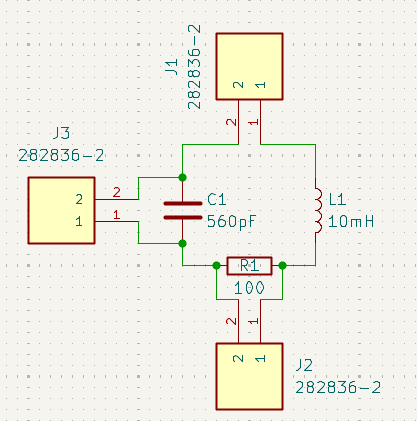
\includegraphics[width=0.978\textwidth]{Figures/02_06_2025/Schematic_borneras}
					\captionsetup{width=0.8\textwidth}
					\subcaption{}
				\end{subfigure}
		\end{minipage}\begin{minipage}[c]{0.332149\textwidth}
			\begin{subfigure}{\textwidth}
					\centering
					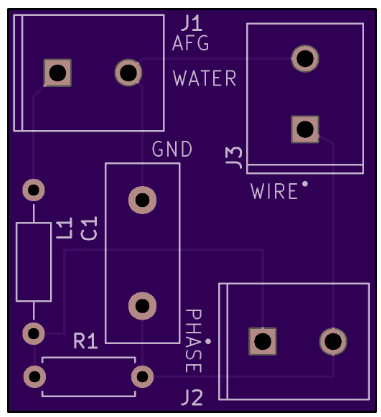
\includegraphics[width=0.978\textwidth]{Figures/02_06_2025/PCB_Top_borneras.png}
					\captionsetup{width=0.8\textwidth}
					\subcaption{}
				\end{subfigure}
		\end{minipage}\begin{minipage}[c]{0.3321249\textwidth}
		\begin{subfigure}{\textwidth}
			\centering
			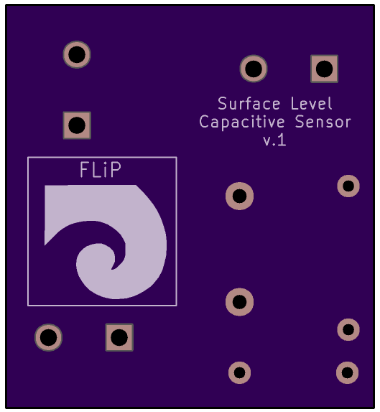
\includegraphics[width=0.978\textwidth]{Figures/02_06_2025/PCB_Bottom_borneras}
			\captionsetup{width=0.8\textwidth}
			\subcaption{}
		\end{subfigure}
	\end{minipage}
	\caption{A la izquierda el esquema del circuito eléctrico que corresponde a la placa. A la derecha la vista superior e inferior de la placa terminada.} %  y  
	\label{fig:}
\end{figure}




\begin{figure}[!ht]
	\begin{minipage}[c]{0.5\textwidth}
			\begin{subfigure}{\textwidth}
					\centering
					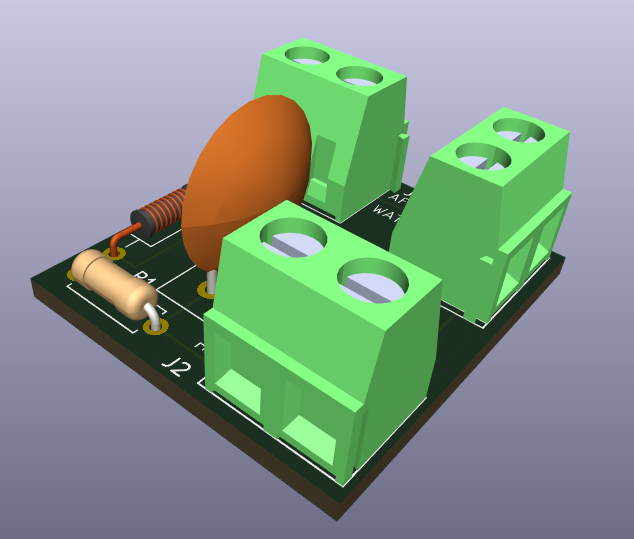
\includegraphics[width=0.82\textwidth]{Figures/02_06_2025/PCB_3D_perfil_borneras1}
					\captionsetup{width=0.8\textwidth}
					\subcaption{}
				\end{subfigure}
		\end{minipage}\begin{minipage}[c]{0.49\textwidth}
			\begin{subfigure}{\textwidth}
					\centering
					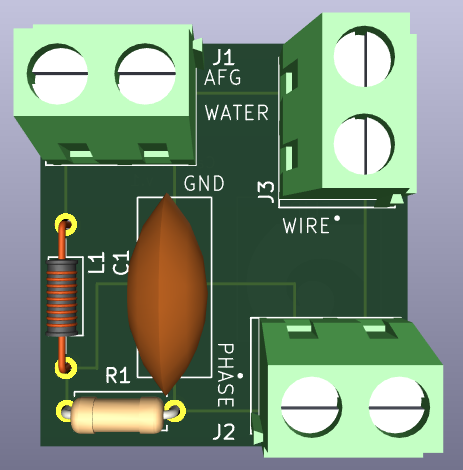
\includegraphics[width=0.78\textwidth]{Figures/02_06_2025/PCB_3D_top_borneras}
					\captionsetup{width=0.8\textwidth}
					\subcaption{}
				\end{subfigure}
		\end{minipage}
	\caption{Dos vistas del Modelo 3D de la placa con sus componentes.}
	\label{fig:}
\end{figure}

La placa terminada tiene dimensiones 26.0 x 28.5mm. El costo estimado de 3 placas debería ser USD 5.70 según OSHPARK. % $ $ 

% 5 Figures/02_06_2025/PCB_Bottom_borneras
% Figures/02_06_2025/PCB_Top_BNC

\section{PCB con BNC.}
\begin{figure}[!ht]
	\begin{minipage}[c]{0.3325\textwidth}
		\begin{subfigure}{\textwidth}
			\centering
			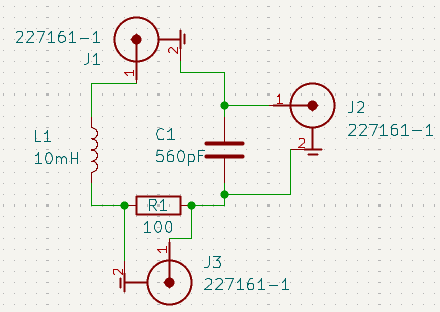
\includegraphics[width=0.978\textwidth]{Figures/02_06_2025/Schematic_BNC}
			\captionsetup{width=0.8\textwidth}
			\subcaption{}
		\end{subfigure}
	\end{minipage}\begin{minipage}[c]{0.332149\textwidth}
		\begin{subfigure}{\textwidth}
			\centering
			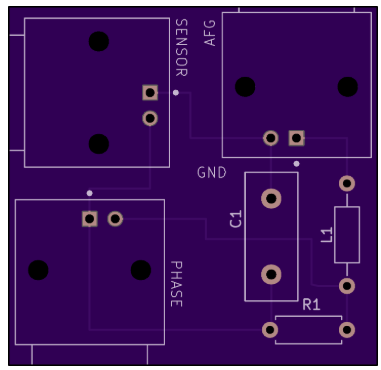
\includegraphics[width=0.978\textwidth]{Figures/02_06_2025/PCB_Top_BNC.png}
			\captionsetup{width=0.78\textwidth}
			\subcaption{}
		\end{subfigure}
	\end{minipage}\begin{minipage}[c]{0.3321249\textwidth}
		\begin{subfigure}{\textwidth}
			\centering
			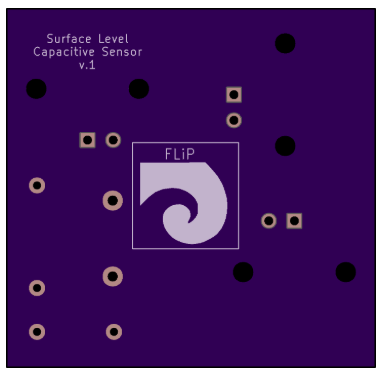
\includegraphics[width=0.978\textwidth]{Figures/02_06_2025/PCB_Bottom_BNC}
			\captionsetup{width=0.8\textwidth}
			\subcaption{}
		\end{subfigure}
	\end{minipage}
	\caption{A la izquierda el esquema del circuito eléctrico que corresponde a la placa. A la derecha la vista superior e inferior de la placa terminada.}
	\label{fig:}
\end{figure}





\begin{figure}[!ht]
	\begin{minipage}[c]{0.5\textwidth}
		\begin{subfigure}{\textwidth}
			\centering
			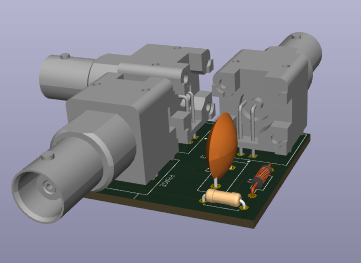
\includegraphics[width=0.98\textwidth]{Figures/02_06_2025/PCB_3D_perfil_BNC}
			\captionsetup{width=0.8\textwidth}
			\subcaption{}
		\end{subfigure}
	\end{minipage}\begin{minipage}[c]{0.49\textwidth}
		\begin{subfigure}{\textwidth}
			\centering
			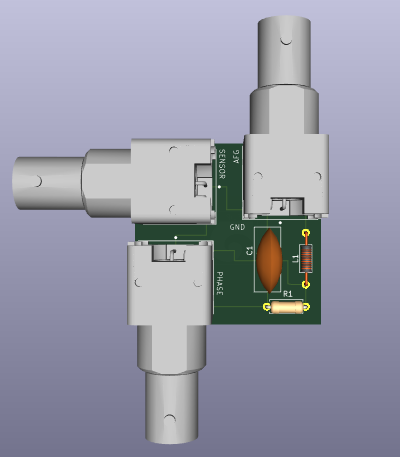
\includegraphics[width=0.8\textwidth,angle=90,origin=c]{Figures/02_06_2025/PCB_3D_top_BNC}
			\captionsetup{width=0.8\textwidth}
			\subcaption{}
		\end{subfigure}
	\end{minipage}
	\caption{Dos vistas del Modelo 3D de la placa con sus componentes.}
	\label{fig:}
\end{figure}



Las dimensiones de la placa son 36.5 x 35.5mm. El costo de 3 placas debería ser USD 10.05 según OSHPARK. % $ $

\section{Componentes.}
Los componentes para las placas son las resistencias, capacitancias e inductancias que ya tenemos en el Laboratorio, los agujeros se eligieron según el pin pitch y dimensiones de estos. Después para las conexiones al exterior se utilizarían:

\begin{itemize}
	\item Bornera de 2 pines: TE Connectivity 282836-2 de ELEMON.
	\item Jack BNC-PCB 90°: de iUrbaNet, el modelo que declaran no lo encontré, así que usé las plantillas del de TE Connectivity 227161-1.
\end{itemize}
